%%%%%%%%%%%%%%%%%%%%%%%%%%%%%%%%%%%%%%%%%%%%%%%%%%%%%%%%%%%%%%%%%%%%%%
%     File: ExtendedAbstract_resul.tex                               %
%     Tex Master: ExtendedAbstract.tex                               %
%                                                                    %
%     Author: Andre Calado Marta                                     %
%     Last modified : 27 Dez 2011                                    %
%%%%%%%%%%%%%%%%%%%%%%%%%%%%%%%%%%%%%%%%%%%%%%%%%%%%%%%%%%%%%%%%%%%%%%
% Results
% Results should be clear and concise.
% Discussion
% This should explore the significance of the results of the work, not
% repeat them. A combined Results and Discussion section is often
% appropriate. Avoid extensive citations and discussion of published
% literature.
%%%%%%%%%%%%%%%%%%%%%%%%%%%%%%%%%%%%%%%%%%%%%%%%%%%%%%%%%%%%%%%%%%%%%%

\section{Results}
\label{sec:resul}

%- Cutflow table \\
%- ...

The analysis described in section \ref{sec:imple} was developed and optimized using samples simulated with the default FCC-hh detector implementation. The results are reported in terms of the significance, $S/\sqrt{B}$, that was achieved (section \ref{sec:results_FCC}). The same analysis is applied to the different detector configurations (described in section \ref{sec:sim}) and the results compared in terms of significance and signal efficiency (section \ref{sec:gran_studies}).  

\subsection{Higgs pair discovery potential at the FCC-hh}
\label{sec:results_FCC}

Considering the SM signal production the achieved significance is
\begin{equation}
	(S/\sqrt{B})_{SM}=8.8\pm 1.6~\text{(stat.)}~^{+4.4}_{-3.4}~\text{(sys.)}
\end{equation}
for an integrated luminosity of $30~\text{ab}^{-1}$. The value of the significance is above the observation threshold which indicates that the full dataset expected to be accumulated in the FCC-hh should be enough to declare the observation (or to exclude) the production of Higgs pairs as predicted by the SM.

For the $1$ TeV DM mediator signal, the significance is $2.3\pm0.4~\text{(stat.)}~^{+1.2}_{-0.9}~\text{(sys.)}$ for $\mathcal{L}=30~\text{ab}^{-1}$ which makes it a challenging and probably inaccessible benchmark. For the 2HDM signal the achieved significance is 
\begin{equation}
	(S/\sqrt{B})_{2HDM}=16.9\pm 3.0~\text{(stat.)}~^{+8.5}_{-6.6}~\text{(sys.)}
\end{equation}
for $\mathcal{L}=30~\text{ab}^{-1}$, making it a very interesting benchmark model from the point of view of enhancing Higgs pair production with respect to the SM. 

The signal efficiency is higher for both BSM models than for the SM, because the masses of the new heavy resonances were chosen to be large ($O(1 ~\text{TeV})$), so as to produce highly boosted Higgs pairs. For the SM the efficiency is approximately $0.4\%$. It increases to $0.5\%$ for the DM mediator model and to $1.7\%$ for the 2HDM. 

\subsection{Granularity studies for future colliders}
\label{sec:gran_studies}

Figure \ref{fig:eff_gran} shows the signal efficiency (in percentage) as a function of the detector configuration. The left most point corresponds to the ATLAS detector and the right most point to the FCC-hh detector with a granularity twice as good in $\eta$ and $\phi$ (configuration 5 in table \ref{table:Gran}). The points in between are ordered by increasing granularity of the HCAL. All other plots that show some quantity as a function of detector configuration follow the same convention. For all signal models, the efficiency increases as the granularity of the HCAL increases. It increases by approximately $30\%$ from the first to the last points.

Figures \ref{fig:SSB_gran} and \ref{fig:SSB_gran_2HDM} show the significance as a function of the detector configuration for the SM signal model and for the 2HDM, respectively. Triangular markers represent analyses that were performed using pure HCAL jets, while square markers represent analysis performed using energy flow jets. 

For energy flow jets the change in significance is very mild. It varies by approximately $30\%$ between the first and last points, for both signal models. It becomes more pronounced when using pure calorimeter jets. In this case, it varies by approximately $70\%~(55\%)$ between the first and last points for the SM (2HDM) signal. However, when using calorimeter jets, the achieved significance is always smaller (for the same detector configuration) because we are not using information from the tracking system. This is verified for both the SM and 2HDM signals. These results indicate that when using energy flow jets the tracking system is dominating the jet reconstruction.

The discussion of some caveats is now in order. In Delphes, it is assumed that it is always convenient to estimate the momentum of charged particles via the tracker, while in a real experiment the energy resolution of the tracking system is only better than that of the calorimeter up to a given energy threshold \cite{Delphes}. In addition, in Delphes, the transverse segmentation of the tracking system is considered to be infinitely small, which is a good approximation but does not exactly reproduce what happens in a real experiment. This might indicate that the results obtained in this work using particle flow jets are overly optimistic. Conversely, the jet reconstruction algorithm for calorimeter jets, as implemented in Delphes, is overly simplistic because no longitudinal segmentation of the calorimeter is considered and no topological algorithm is used. This might indicate that the results obtained in this work using calorimeter jets are overly pessimistic.

All in all, performing this or similar studies using full detector simulation is of the utmost importance in order to obtain more realistic results that can be used as input for detector optimization studies for future colliders.

\begin{figure}[h]
	\centering
	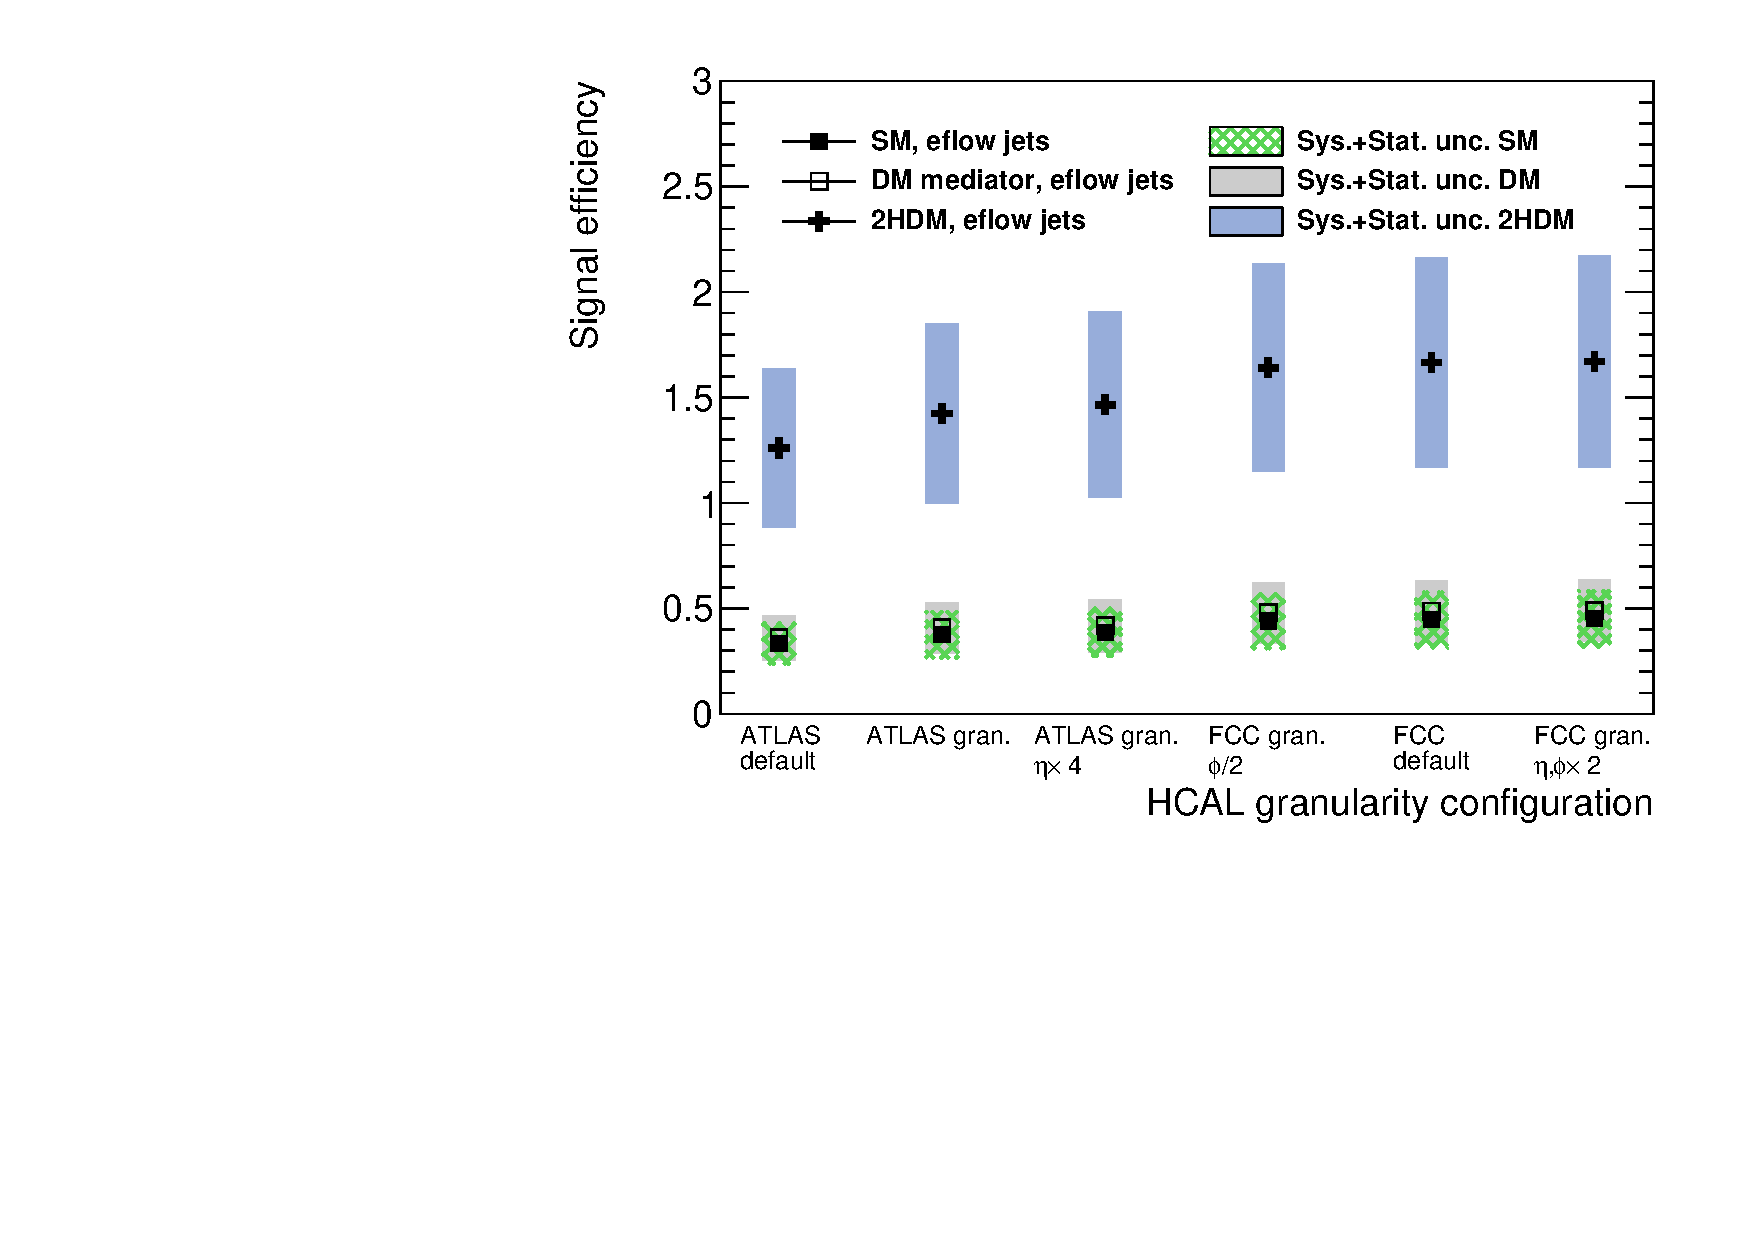
\includegraphics[width=\linewidth]{./images/EffvsGran_PFjets_Opt.pdf}
	\caption{Signal efficiency in percentage as a function of the detector configuration. The statistical error bars are drawn but are smaller than the markers.}
	\label{fig:eff_gran}
\end{figure}

\begin{figure}[h]
	\centering
	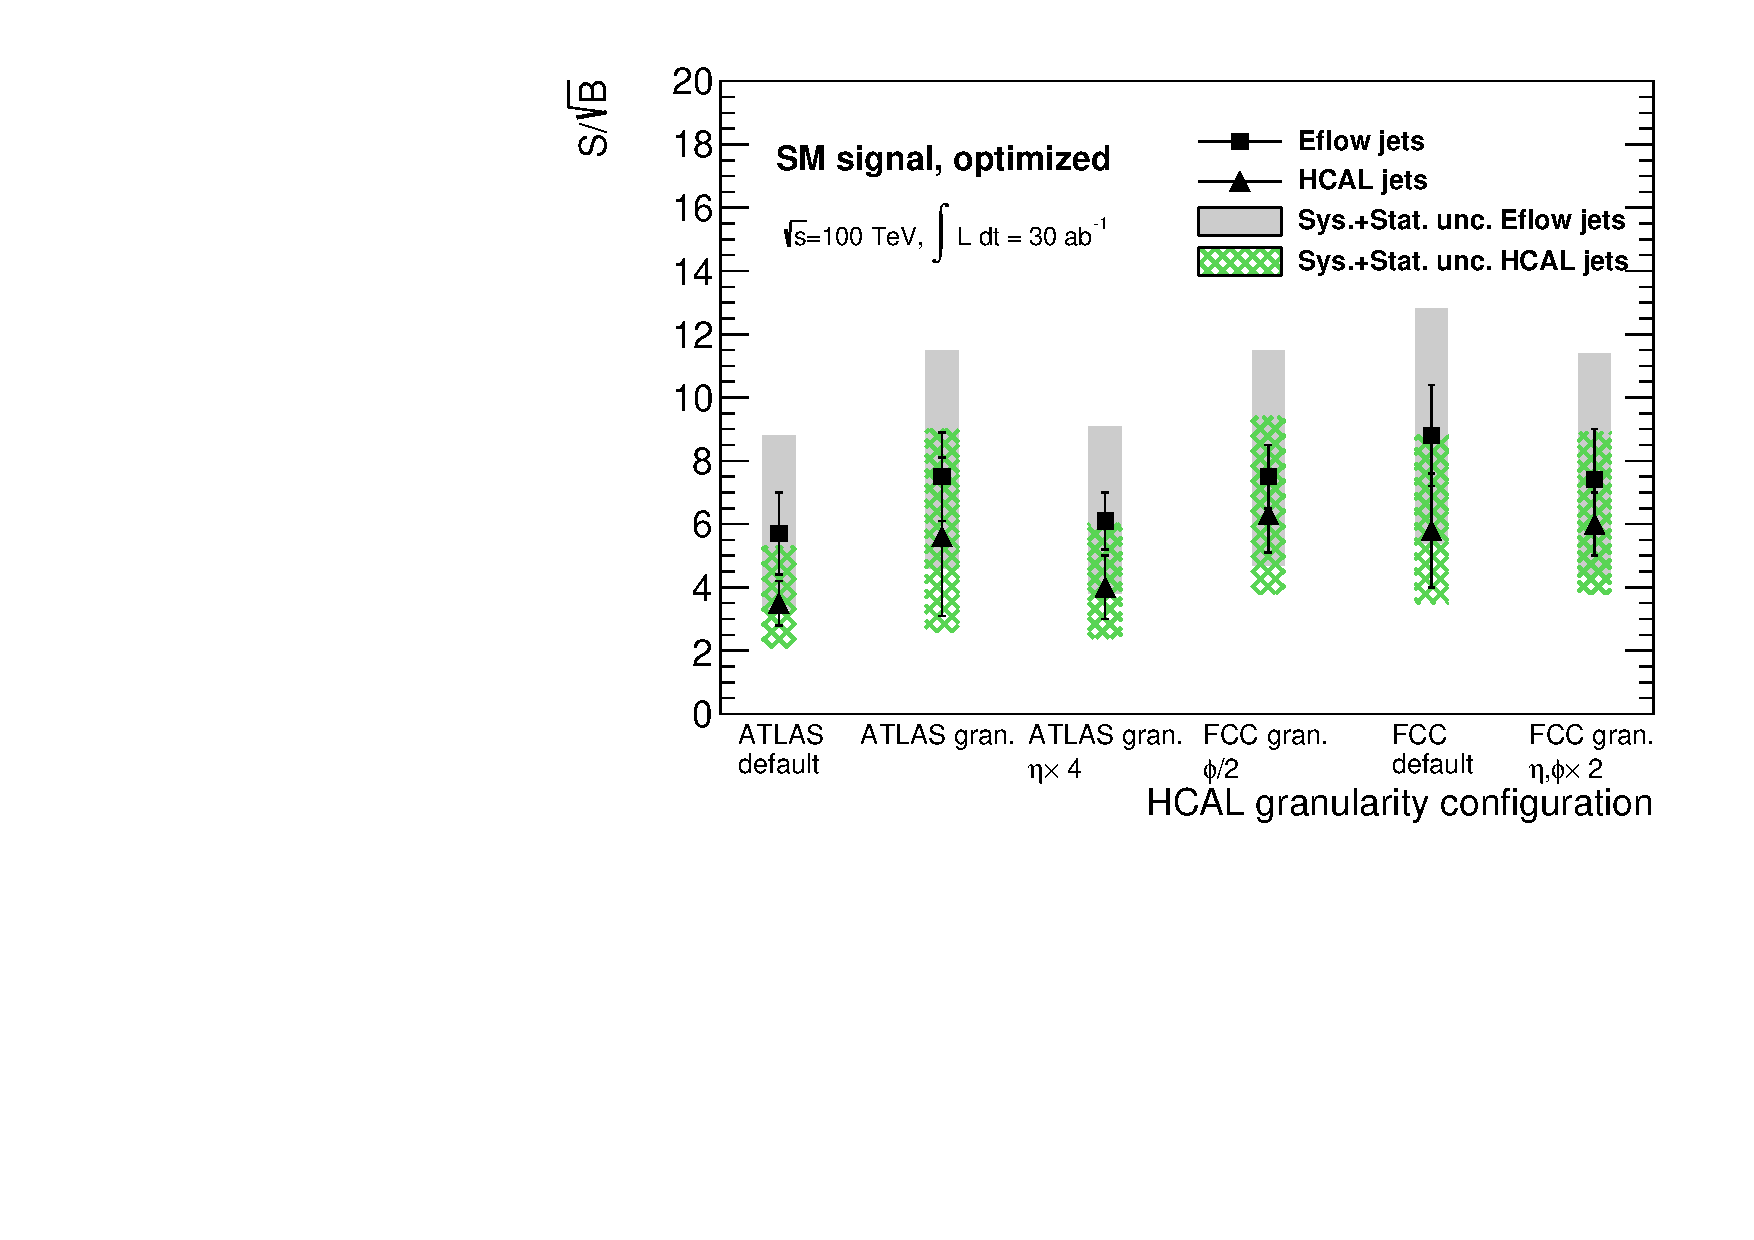
\includegraphics[width=\linewidth]{./images/SSBvsGran_SM_Opt.pdf}
	\caption{$S/\sqrt{B}$ as a function of the detector configuration for the SM signal model. The square (triangular) markers refer to values obtained using particle flow (calorimeter) jets.}
	\label{fig:SSB_gran}
\end{figure}

\begin{figure}[h]
	\centering
	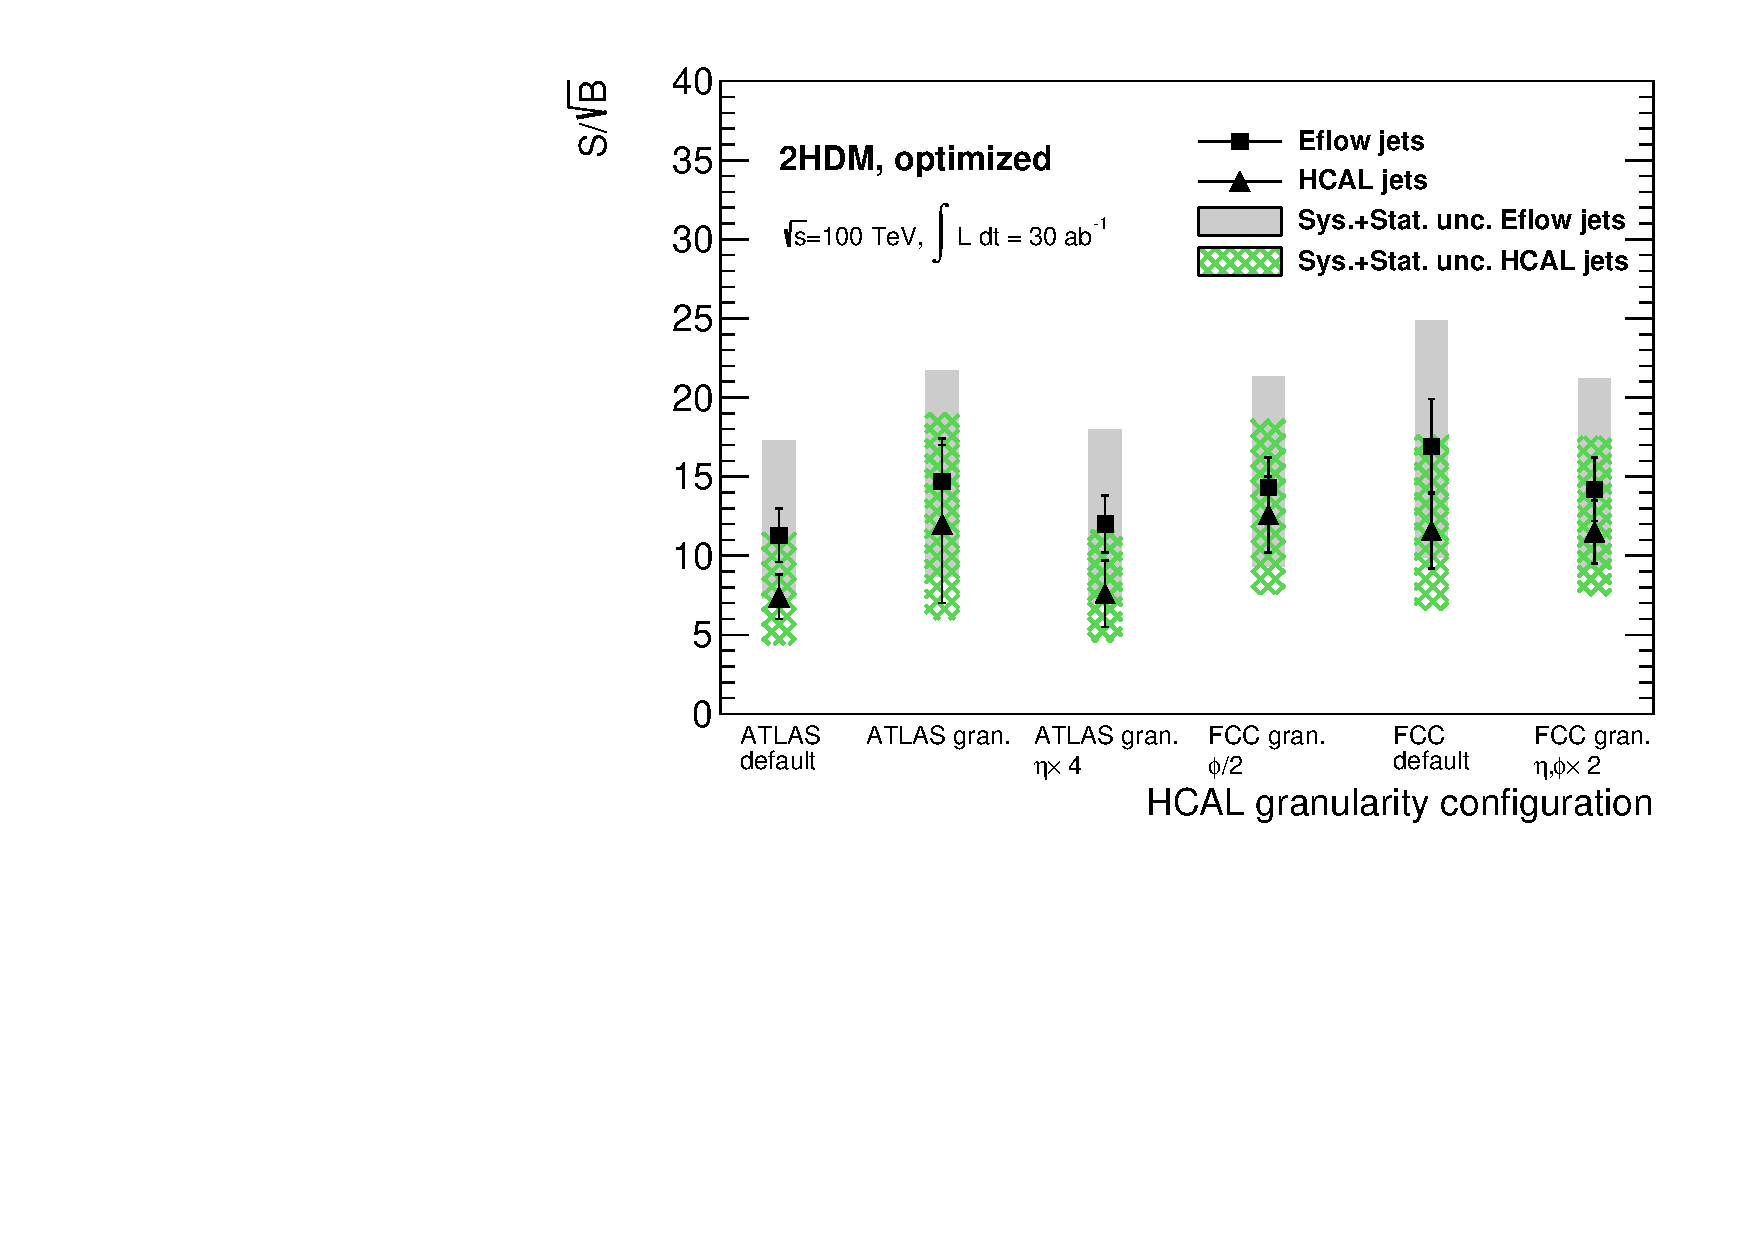
\includegraphics[width=\linewidth]{./images/SSBvsGran_2HDM_Opt.pdf}
	\caption{$S/\sqrt{B}$ as a function of the detector configuration for the 2HDM signal model. The square (triangular) markers refer to values obtained using particle flow (calorimeter) jets.}
	\label{fig:SSB_gran_2HDM}
\end{figure}

